%\documentclass[pdftex,a4paper]{scrreprt}
\documentclass[fleqn,pdftex,paper=a4,pagesize,11pt,numbers=noenddot]{scrreprt}
\usepackage[intoc]{nomencl}
\usepackage[numbers]{natbib}
\usepackage{booktabs}
\usepackage{geometry}
\usepackage{multirow}
\usepackage{multicol}
\usepackage{booktabs}
\usepackage{fancyhdr}
\usepackage{array}

\usepackage[nottoc]{tocbibind}

\usepackage[T1]{fontenc}
\setcounter{tocdepth}{3}


\usepackage{algorithmicx}
\usepackage{algorithm}
\usepackage{algpseudocode}
\floatname{algorithm}{Procedure}

%\usepackage[automark]{scrpage2}
\usepackage{cite}

\usepackage[dvips]{color}
\usepackage{epsfig}
\usepackage{grffile}
\usepackage{epstopdf}
\usepackage{ae}

\usepackage{amsmath}
\usepackage{amssymb}
\usepackage{amsfonts}
\usepackage{amsthm}
\usepackage{mathtools}

\usepackage{float}
\usepackage{graphics}
\usepackage{graphicx, subfigure}
\setcounter{lofdepth}{2}
\graphicspath{{/Volumes/workspace/studium/bachelorarbeit/thesis/media/}}
\newcommand{\rulesep}{\unskip\ \vrule\ }
\newcommand{\rpm}{\sbox0{$1$}\sbox2{$\scriptstyle\pm$}
  \raise\dimexpr(\ht0-\ht2)/2\relax\box2 }

\usepackage{titlepage}

\usepackage{appendix}

\usepackage{pstricks}

\pagestyle{headings}

\usepackage{ifthen}
\makenomenclature
\makeindex
\setlength{\nomlabelwidth}{.25\hsize}
%\renewcommand{\nomlabel}[1]{#1 \dotfill}
\setlength{\nomitemsep}{-\parsep}

\renewcommand{\nomgroup}[1]{%
\renewcommand{\makelabel}[1][]{##1}
\item[~]
\ifthenelse{\equal{#1}{A}}{\item[\lARGE\textbf{Abbreviations}]}{
\ifthenelse{\equal{#1}{B}}{\item[\lARGE\textbf{Operators and Symbols}]}{
\ifthenelse{\equal{#1}{C}}{\item[\lARGE\textbf{Superscripts and Subscripts}]}{
\ifthenelse{\equal{#1}{D}}{\item[\lARGE\textbf{Domains and boundaries}]}{
\ifthenelse{\equal{#1}{E}}{\item[\lARGE\textbf{Kinematics}]}{
\ifthenelse{\equal{#1}{F}}{\item[\lARGE\textbf{Stresses and constitutive laws}]}{
\ifthenelse{\equal{#1}{G}}{\item[\lARGE\textbf{Governing equations}]}{
\ifthenelse{\equal{#1}{H}}{\item[\lARGE\textbf{Contact Mechanics}]}{
\ifthenelse{\equal{#1}{I}}{\item[\lARGE\textbf{Numerical methods}]}{}}}}}}}}}
\item[~]
\let\makelabel\nomlabel
}


\DeclareMathOperator{\tr}{tr}
\DeclareMathOperator{\Div}{Div}
\DeclareMathOperator{\Lin}{Lin}
\DeclareMathOperator{\divnew}{div}
\DeclareMathOperator{\Grad}{Grad}
\DeclareMathOperator{\tonew}{to}
\DeclareMathOperator{\innew}{in}
\DeclareMathOperator{\on}{on}
\DeclareMathOperator{\subjectnew}{subject}


\makeindex

%%%%%%%%%%%%%%%%%%%%%%%%%%%%%%%%%%%%%%%%%%%%%%%%%%%%%%%%%%%%%%%%%%%%%%%
%%%%%%%%%%%%%%%%%%%%%%%%%%%%             %%%%%%%%%%%%%%%%%%%%%%%%%%%%%%
%%%%%%%%%%%%%%%%%%%%%%%%%%%% end of file %%%%%%%%%%%%%%%%%%%%%%%%%%%%%%
%%%%%%%%%%%%%%%%%%%%%%%%%%%%             %%%%%%%%%%%%%%%%%%%%%%%%%%%%%%
%%%%%%%%%%%%%%%%%%%%%%%%%%%%%%%%%%%%%%%%%%%%%%%%%%%%%%%%%%%%%%%%%%%%%%%

\usepackage{hyperref}
\usepackage{bookmark}
\usepackage{multirow}
\usepackage{rotating}

%%
\usepackage[framemethod=tikz]{mdframed}
\usetikzlibrary{calc}
\usepackage{kantlipsum}

%\usepackage{dingbat}%\eye and \leftpointright

\newcounter{error}[chapter]
\renewcommand*\theerror{\thechapter.\arabic{error}}
\tikzset{
errorsymbol/.style={%
    rectangle,draw=blue,
   ,scale=2,overlay}}

\tikzstyle{line} = [ draw, -latex']  
\usetikzlibrary{calc}

\tikzset{
 lampsymbol/.style={%
   ,scale=2,overlay}}

\newmdenv[hidealllines=true,backgroundcolor=blue!5,%
 frametitle={\stepcounter{error}Comman~Programming~Error~\theerror},
 frametitlefont=\color{blue!80!black}\bfseries,
 skipabove=\topsep,skipbelow=\topsep,nobreak,
 leftmargin=.3cm,rightmargin=.3cm, innerleftmargin=2cm,
 singleextra={\path let \p1=(P), \p2=(O) in ($(\x2,0)+0.5*(2,\y1)$) node[errorsymbol] {aaa};},%
]{error}


\newmdenv[nobreak,middlelinewidth=.8pt,
 frametitlefont=\bfseries,
 leftmargin=.3cm,rightmargin=.3cm, innerleftmargin=2cm,
 skipabove=\topsep,skipbelow=\topsep,
 singleextra={\path let \p1=(P), \p2=(O) in ($(\x2,0)+0.5*(2,\y1)$) node[ lampsymbol] {.h};
                          \draw[line width=.8pt,white,] ($(O|-P)+(.2cm,0)$) -- ($(P)-(.2cm,0)$); 
                          \draw[line width=.8pt,white,] ($(O)+(.2cm,0)$) -- ($(P|-O)-(.2cm,0)$);
    },%
]{bbbb}

\newcommand{\infobox}[1]{\begin{bbbb}[frametitle={Reference to NS-EOF namespaces}]#1\end{bbbb}}



%%

%%
\usepackage{lscape}
%\usepackage{adjustbox}
%%

\usepackage{etex}
\newcounter{alteSeitenzahl}

\usepackage{tikz}
\usetikzlibrary{shapes,arrows,chains}
\usepackage{xcolor}

\usepackage{graphicx}
%\usepackage[usenames,dvipsnames,svgnames,table]{xcolor}

\usepackage{dirtree}
\usepackage{epstopdf}
\usepackage{textcomp}
\usepackage[final]{listings}
\definecolor{lightgray}{rgb}{.7,.7,.7}
\definecolor{gray}{rgb}{.4,.4,.4}
\definecolor{darkblue}{rgb}{0,0,.3}

\newcommand{\noi}{\noindent}
\newcommand{\noii}{\vspace{3mm}\noindent}

\newcommand{\abl}[2]{\frac{\partial\,#1}{\partial\,#2}}
\newcommand{\abll}[2]{\frac{\partial^2\,#1}{\partial\,#2^2}}
\newcommand{\ave}[1]{\left\langle #1 \right\rangle}
\newcommand{\new}[1]{\textcolor{red}{#1}}

%\lstset{
%showstringspaces=false,
%extendedchars=true,
%frameround=fttt,
%frame=single,
%upquote=true,
%breaklines=true
%}

\newcommand{\ke}{$k$-$\varepsilon$}

\newcommand{\xmll}[2]{
    \lstset{
numberstyle=\tiny,%5
basicstyle={\ttfamily},%
    language=xml,
    %tabsize=3,
    %frame=lines,
    %caption=Test,
    %label=code:sample,
    %frame=shadowbox,
    %rulesepcolor=\color{gray},
    %xleftmargin=20pt,
    %framexleftmargin=15pt,
    frame=single,
    keywordstyle=\color{blue}\bf,
    commentstyle=\color{OliveGreen},
    stringstyle=\color{red},
    numbers=left,
    numberstyle=\tiny,
    %numbersep=5pt,
    breaklines=true,
    showstringspaces=false,
    %basicstyle=\footnotesize,
    emph={food,name,price},emphstyle={\color{magenta}}}
\lstinputlisting[firstline=#2]{#1}}

\newcommand{\bashh}[2]{
    \lstset{
numberstyle=\tiny,%5
basicstyle={\ttfamily},%
    language=xml,
    %tabsize=3,
    %frame=lines,
    %caption=Test,
    %label=code:sample,
    %frame=shadowbox,
    %rulesepcolor=\color{gray},
    %xleftmargin=20pt,
    %framexleftmargin=15pt,
    frame=single,
    keywordstyle=\color{blue}\bf,
    commentstyle=\color{OliveGreen},
    stringstyle=\color{red},
    numbers=left,
    numberstyle=\tiny,
    %numbersep=5pt,
    breaklines=true,
    showstringspaces=false,
    %basicstyle=\footnotesize,
    emph={food,name,price},emphstyle={\color{magenta}}}
\lstinputlisting[firstline=#2]{#1}}

\begin{document}





%\pagestyle{useheadings}
\pagenumbering{roman}


\thesistype{Project Report}
\author{Marten Lienen, Peter M\"unch, Walter Simson, Josef Winter}
\matno{ a}
\title{$k$-$\varepsilon$ Turbulence Model}
\tutor{ b}{ c}


\maketitle
\newpage
\thispagestyle{empty}
\quad
\newpage

\tableofcontents
\printnomenclature
\newpage

\setcounter{alteSeitenzahl}{\value{page}}
\pagenumbering{arabic}

\chapter{Introduction} % (fold)
\label{cha:introduction}

% Peter


The k-$\varepsilon$-turbulence model was implemented part of the lab course 'Turbulent Flow Simulation on HPC-Systems'. For the purpose of efficiency, stability and testing a literature study was performed and following aspects have been considered and added to the existing code framework:

\begin{itemize}
\item wall models
\item new scenarios
\item PETSc optimization
\item adaptive time stepping
\item restart point \& initialisation of the pressure field in PETSc.
\end{itemize}

\noi Results were compared to literature: the wall near velocities (linear and logarithmic layer) matched well with the expected profile. The terms of the transport equations were predicted qualitatively well due to the chosen wall model (Chien).

\noii Furthermore comparisons of the DNS results with measurement results were conducted for a backwards facing step scenario and a flow around a cylinder (Karman Vortex Street).
High emphasis was put on the stochastic evaluation. To be able to simulate a flow around a circle the possibility of importing any arbitrary geometry was implemented.

\noii Extensive thoughts were made how to structure the files of each project in an optimal way (usability \& later clarity).

% chapter introduction (end)
\nomenclature[A]{CPP}{Closest point projection}
\nomenclature[A]{FE}{Finite element}
\nomenclature[A]{FEM}{Finite element method}

\chapter{Turbulence modeling with k-Epsilon model} % (fold)
\label{cha:turbulence_modeling_with_k_epsilon_model}

Josef

\section{Governing equations} % (fold)
\label{sec:governing_equations}



\section{RANS equations} % (fold)
\label{sec:rans_equations}

% subsubsection rans_equations (end)

\section{K-epsilon transport equations} % (fold)
\label{sec:k_epsilon_transport_equations}

% subsubsection k_epsilon_transport_equations (end)

% subsection governing_equations (end)

\section{Discretization} % (fold)
\label{sec:discretization}

% subsection discretization (end)

\section{Modification 1: Low-Reynolds models for wall near region} % (fold)
\label{sec:modification_1_low_reynolds_models_for_wall_near_region}

% subsection modification_1_low_reynolds_models_for_wall_near_region (end)

\section{Modification 2: Limitation of source and reaction terms in transport equtions} % (fold)
\label{sec:modification_2_limitation_of_source_and_reaction_terms_in_transport_equtions}

% subsection modification_2_limitation_of_source_and_reaction_terms_in_transport_equtions (end)

\section{Modified equations and discretization} % (fold)
\label{sec:modified_equations_and_discretization}

% subsection modified_equations_and_discretization (end)

% chapter turbulence_modeling_with_k_epsilon_model (end)
\chapter{Algorithm} % (fold)
\label{cha:algorithm}

Peter

\section{Adaptive time stepping} % (fold)
\label{sec:adaptive_time_stepping}

% subsection adaptive_time_stepping (end)

% chapter algorithm (end)
\chapter{Performance, efficiency and further modifications} % (fold)
\label{cha:performance_efficiency_and_further_modifications}

During simulations with the \ke\,model it was seen that the maximal time step size is much smaller than the one of a DNS simulation due to high eddy viscosity (especially near the inlet) and that the simulation takes a long time to reach steady state flow. This leads to very high computational times forcing us to deal with this situation (e.g. reducing the computational time with different methods).

\noii Please note that this section also mentions further modifications not related to the topic.
 
\section{New scenarios} % (fold)
\label{sec:new_scenarios}

All scenarios are working for DNS, algebraic and $k$-$\epsilon$-simulations.

\infobox{
nseof::GlobalBoundaryFactory,\\ nseof::flowmodels::ke:GlobalBoundaryFactory
}

% subsection new_scenarios (end)

\subsection*{Channel section with symmetry boundary condition} % (fold)
\label{sub:channel_section_with_symmetry_boundary_condition}

The top and the back walls of the 'channel'-scenario are replaced by free slip conditions:

\begin{equation}
\abl{u}{n}=0
\qquad
v = 0
\qquad
\left(
\abl{k}{n}=0
\qquad
\abl{\varepsilon}{n}=0
\right)
\end{equation}  

\noii The free slip condition is often imposed along a line or plane of symmetry  thereby reducing in this case the size of the domain where the flow has to be computed by a half respectively by a forth in the 2D and 3D case \citep{griebel1998}. Symmetry is a valid assumption for a channel flow if recirculations are neglected\footnote{Recirculation cannot be captured by RANS. One would need more advanced/expensive turbulence models.}.

\noii By the way: if the x- and y-ratio of a backwards facing step are specified, it is possible to simulate a 2D free jet similar flow\footnote{Free jet is not a symmetrical phenomenon. A symmetric boundary condition leads obviously to non-physical deviation in the results.}.

% subsubsection channel_section_with_symmetry_boundary_condition (end)

\subsection*{Boundary layer over flat plate} % (fold)
\label{sub:boundary_layer_over_flat_plate}

For a 2D-simulation, the top wall of the 'channel'-scenario was replaced with an opening (Neumann boundary condition).

\noii With this scenario, a boundary layer over a flat plat can be modelled provided that the height $y$ is selected big enough compared to the local boundary layer width.

\subsection*{Free} % (fold)
\label{sub:free}

In this scenario, all wall boundary conditions of the 'channel'-scenario were removed and replaced by openings.

\subsection*{Arbitrary geometric obstacles} % (fold)
\label{sub:arbitrary_geometric_obstacles}

In any scenario, an obstacle of any form (see section~\ref{sec:geometry_file}) can be placed into the middle of the flow field. In this way, the free shear flow plane wake can be modelled. The most notable example is the flow around a circle with certain repeating flow patterns behind the obstacle also known as the K\'{a}rm\'{a}n vortex street (see section~\ref{sec:karman_vortex_street_flow_around_a_cylinder_in_a_channel}).

\noii The wall distance manager (a k-D-tree implementation) was extended to handle the new scenarios and arbitrary geometries.


\noii Limitation: 2D and 1 processor.

\infobox{
nseof::geometry::GeometryManager, \\
nseof::WallDistanceManager
}

% subsubsection arbitrary_geometric_obstacles (end)

\newpage
\section{PETSc-optimization} % (fold)
\label{sec:petsc_optimization}

Marten und Walter

% subsection petsc_optimization (end)

\newpage
\section{Restart points} % (fold)
\label{sec:restart_points}

Respart points were created for the pupose of:
\begin{itemize}
\item faster convergence: starting the simulation with a good initial condition
\item security: in the case of a crash or unexpected end of a simulation.
\end{itemize}

\noii At every restart point a backup file (.bak) is created, which can be loaded at the beginning of a simulation and which is used as the initial condition by PETSc. Following variables are written to the file for each simulation type:

\newcommand{\che}{$\checkmark$}

\begin{center}

\newcolumntype{R}[1]{>{\centering\let\newline\\\arraybackslash\hspace{0pt}}m{#1}}

\begin{tabular}{l  R{2cm}R{2cm}R{2cm}}\hline
 & DNS & Algebraic & $k$-$\varepsilon$\\\hline
Pressure $p$                                    & \che & \che &  \che \\
Velocity $u_i$                                  & \che & \che & \che \\\hline
Eddy viscosity $\nu_t$                          &      & \che &  \\
Pressure + TKE $P$                              &      & \che &  \che \\\hline
Turbulent kinetic energy $k$                    &      &      & \che \\
Dissipation rate $\varepsilon$                  &      &      & \che \\
Additional $k$-source term $D$                  &      &      & \che \\
Additional $\varepsilon$-source term Factor $E$ &      &      & \che \\
Factor $f_1$                                    &      &      & \che \\
Factor $f_2$                                    &      &      & \che \\
Factor $f_3$                                    &      &      & \che \\\hline
\end{tabular}

\end{center}
It is possible also to use the backup file of a simulation type for an other one: e.g. DNS simulation can be started for a \ke\, backup file and vice versa. For the another simulation type unknown variables are set to be zero.

\noii Please note that no interpolation function has been implemented: simulations can be only started from backup files with the same number of processors and the same mesh configuration.

\infobox{
nseof::MPIIterator.h, nseof::MPIIteratorReader.h,\\
nseof::MPIIteratorWriter.h, nseof::PetscSolver.h
}


% subsection restart_points (end)

% chapter performance_efficiency_and_further_modifications (end)
\chapter{Validation of k-epsilon-model} % (fold)
\label{cha:validation_of_k_epsilon_model}

\section{Channel flow} % (fold)
\label{sec:channel_flow}

Peter

% subsection channel_flow (end)

\section{Boundary layer} % (fold)
\label{sec:boundary_layer}

Josef

% subsection boundary_layer (end)

% chapter validation_of_k_epsilon_model (end)
\chapter{Performance tests} % (fold)
\label{cha:performance_tests}

Marten und Walter

% chapter performance_tests (end)
\chapter{Numerical results of DNS simulations} % (fold)
\label{cha:numerical_results}

\section{Backward facing step} % (fold)
\label{sec:backward_facing_step}

Numerical results of:
\begin{itemize}
\item DNS-simulations
\item an algebraic simulation
\item a \ke-simulation
\end{itemize}
were compared with experimental results given us by the department for aerodynamics. Because of its transient character, we also performed a stochastic analysis of the DNS simulations. All simulations were performed in 2D.

\subsubsection*{DNS-simulations}

For DNS, 3 simulations with different inlet velocities were performed ($u=3.372,/s$, $=5.295,/s$, $=5.579,/s$).

\noii The flow in the DNS-simulations is highly transient: vortices and secondary vortices are created created periodically behind the step. They are dragged by the main flow down the channel. Also vortices appear at the top wall. To be able to make reasonable conclusions we performed a stochastic analysis. The stochastic moments of the simulation were inserted into the same plot as the ones of the experimental results (see figure~\ref{fig:bfsA}, \ref{fig:bfsB} and \ref{fig:bfsC}). 

\noii It can be well seen that the maximum mean velocity tends to the bottom wall in the experiment after the step. This extreme behaviour could not be encountered in the simulation: the maximum velocity shifts gradually to the middle of the channel\footnote{The integral of the mean velocity over the paths seem to increase with increasing position x. Maybe the assumption of an incompressible flow is not given.}. The mean reattachment length for $u=3.372m/s$ could be determined to be between position D and E. This is much longer as the reattachment length of the experiment.

\noii Please note that the variance at the inlet of the experimental backward facing step is quite high\footnote{No velocity fluctuation was assumed at the inlet of the simulations.}. This and different vortex patterns downstream of the step might be the reason for the discrepancy of the mean flow profile and the attachment length.

\newpage

\begin{figure}[!htb]
\centering
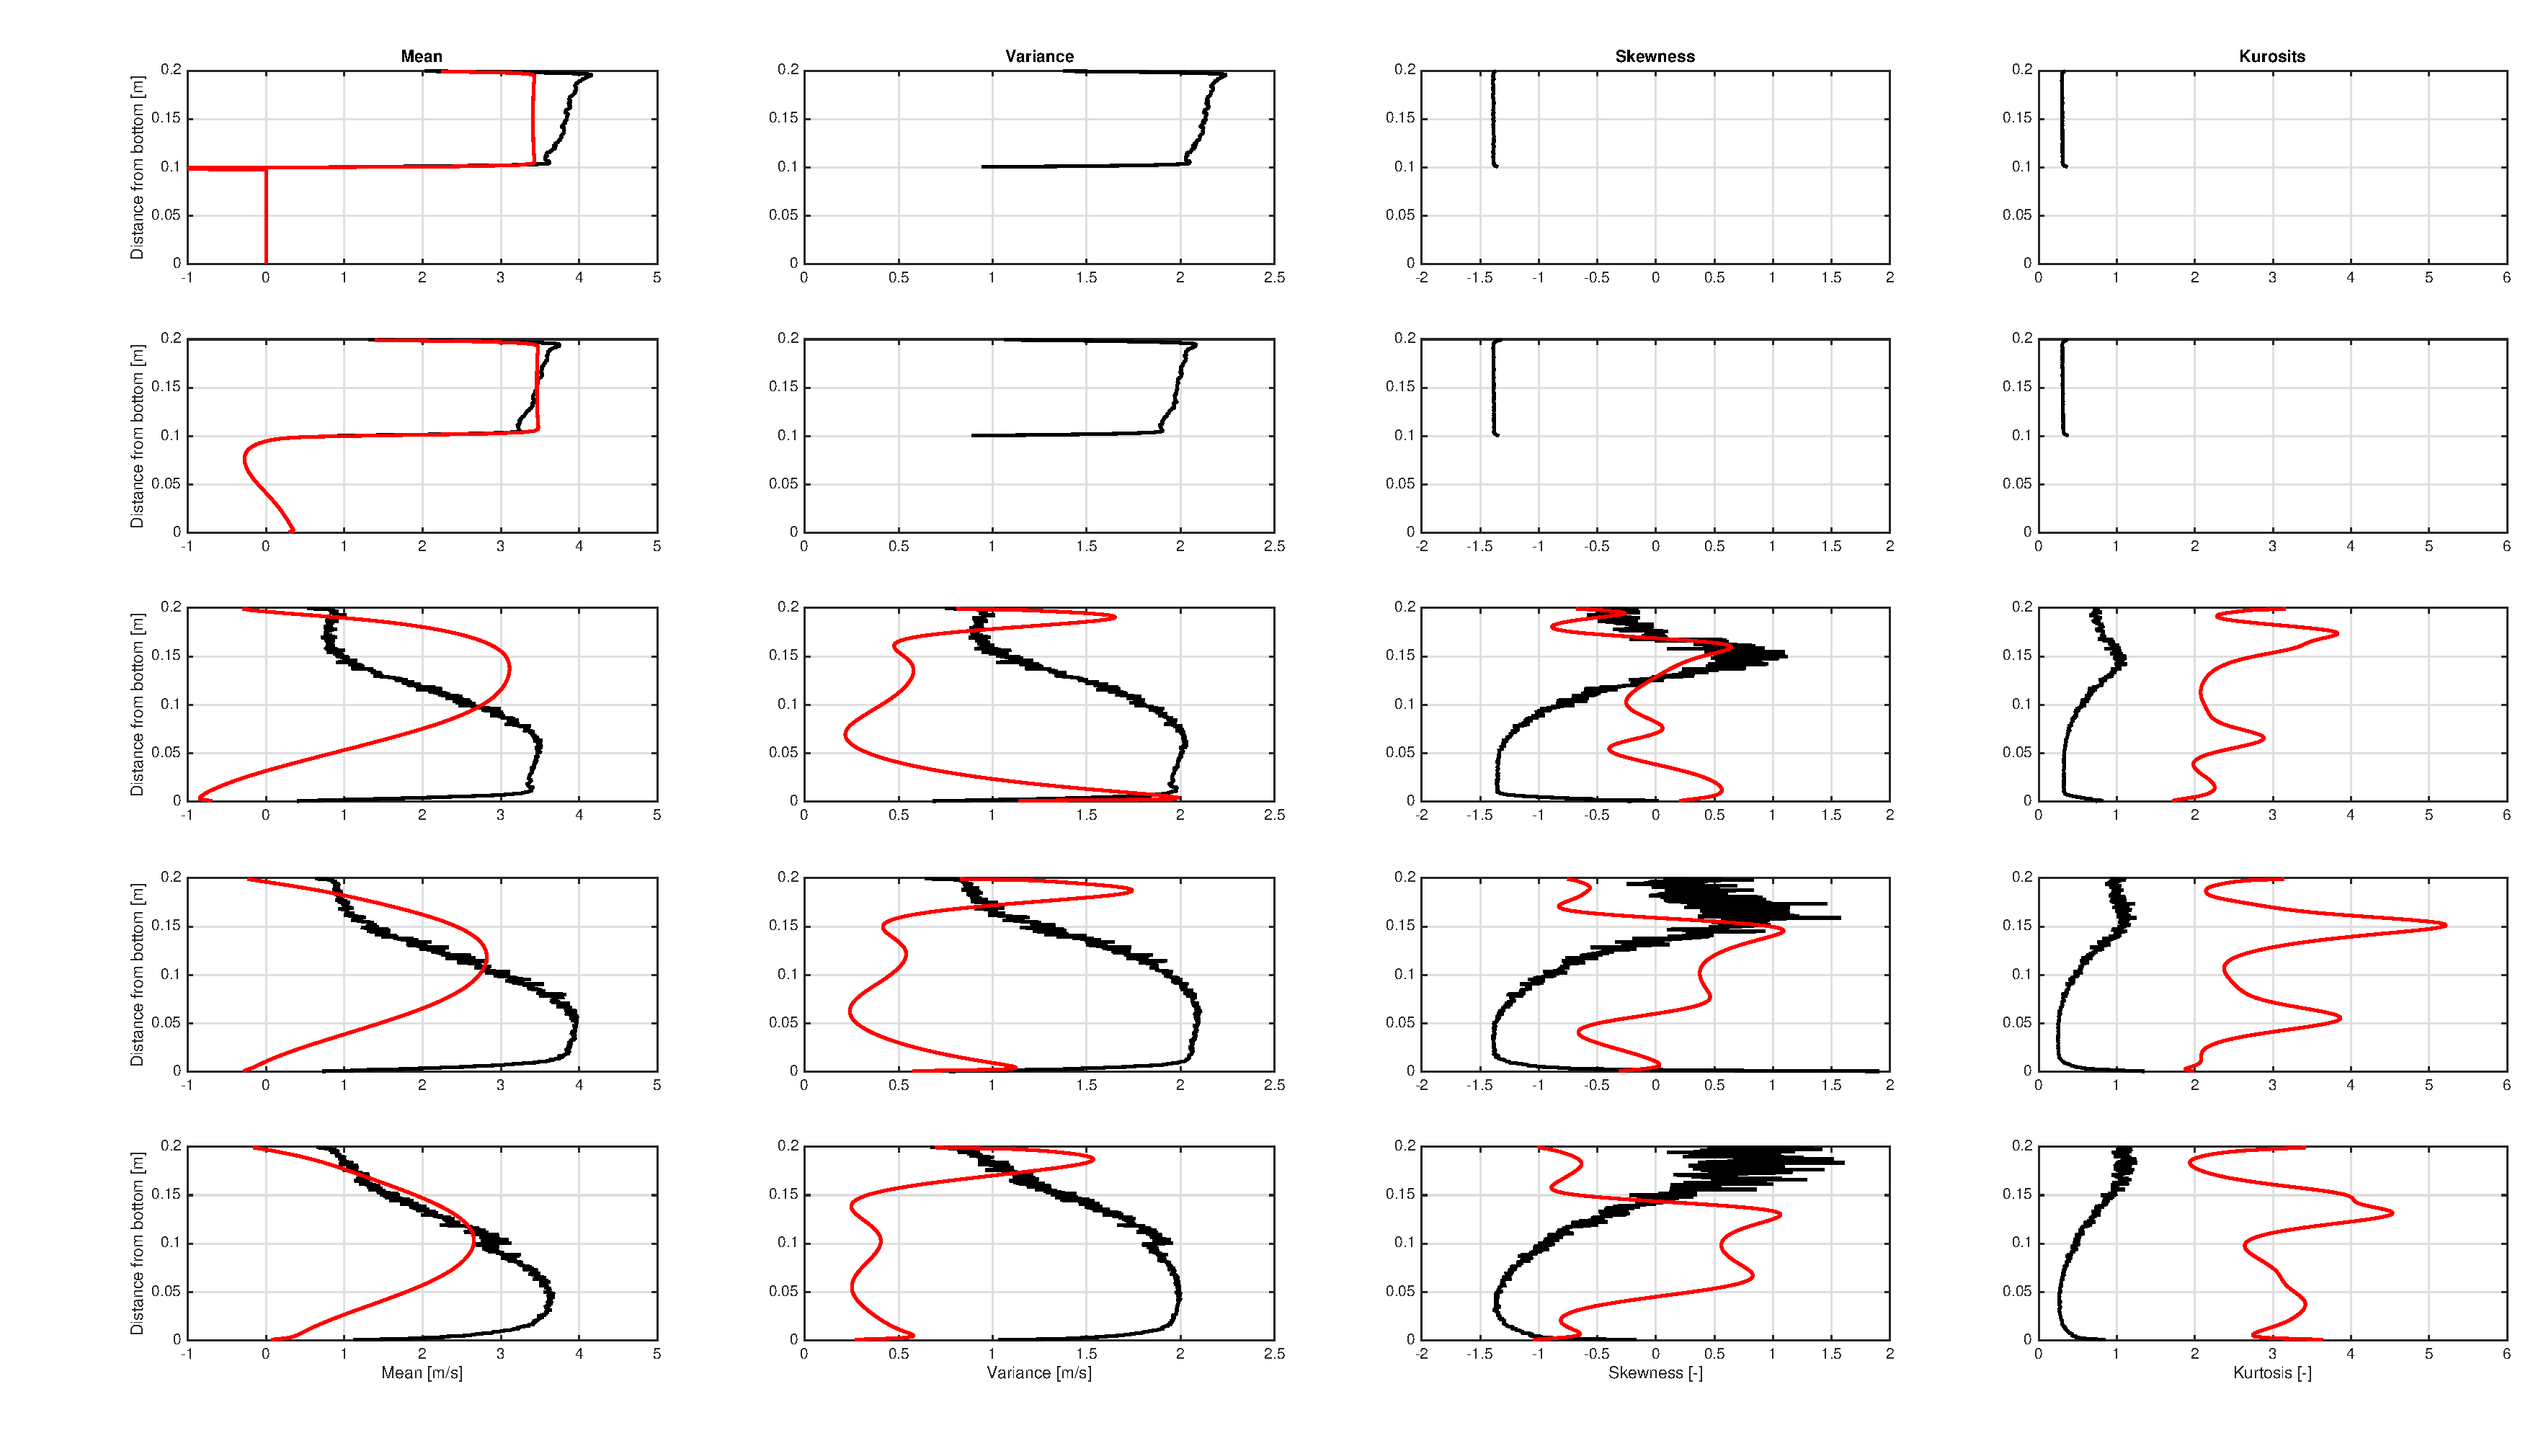
\includegraphics[trim=0 0 0 0,clip,angle=90,width=0.8\textwidth]{FIGURES/Re00_dns.eps}
\caption{Stochastic analysis and comparison for $u=3.372m/s$ for different x-positions}
\label{fig:bfsA}
\end{figure} 

\begin{figure}[!htb]
\centering
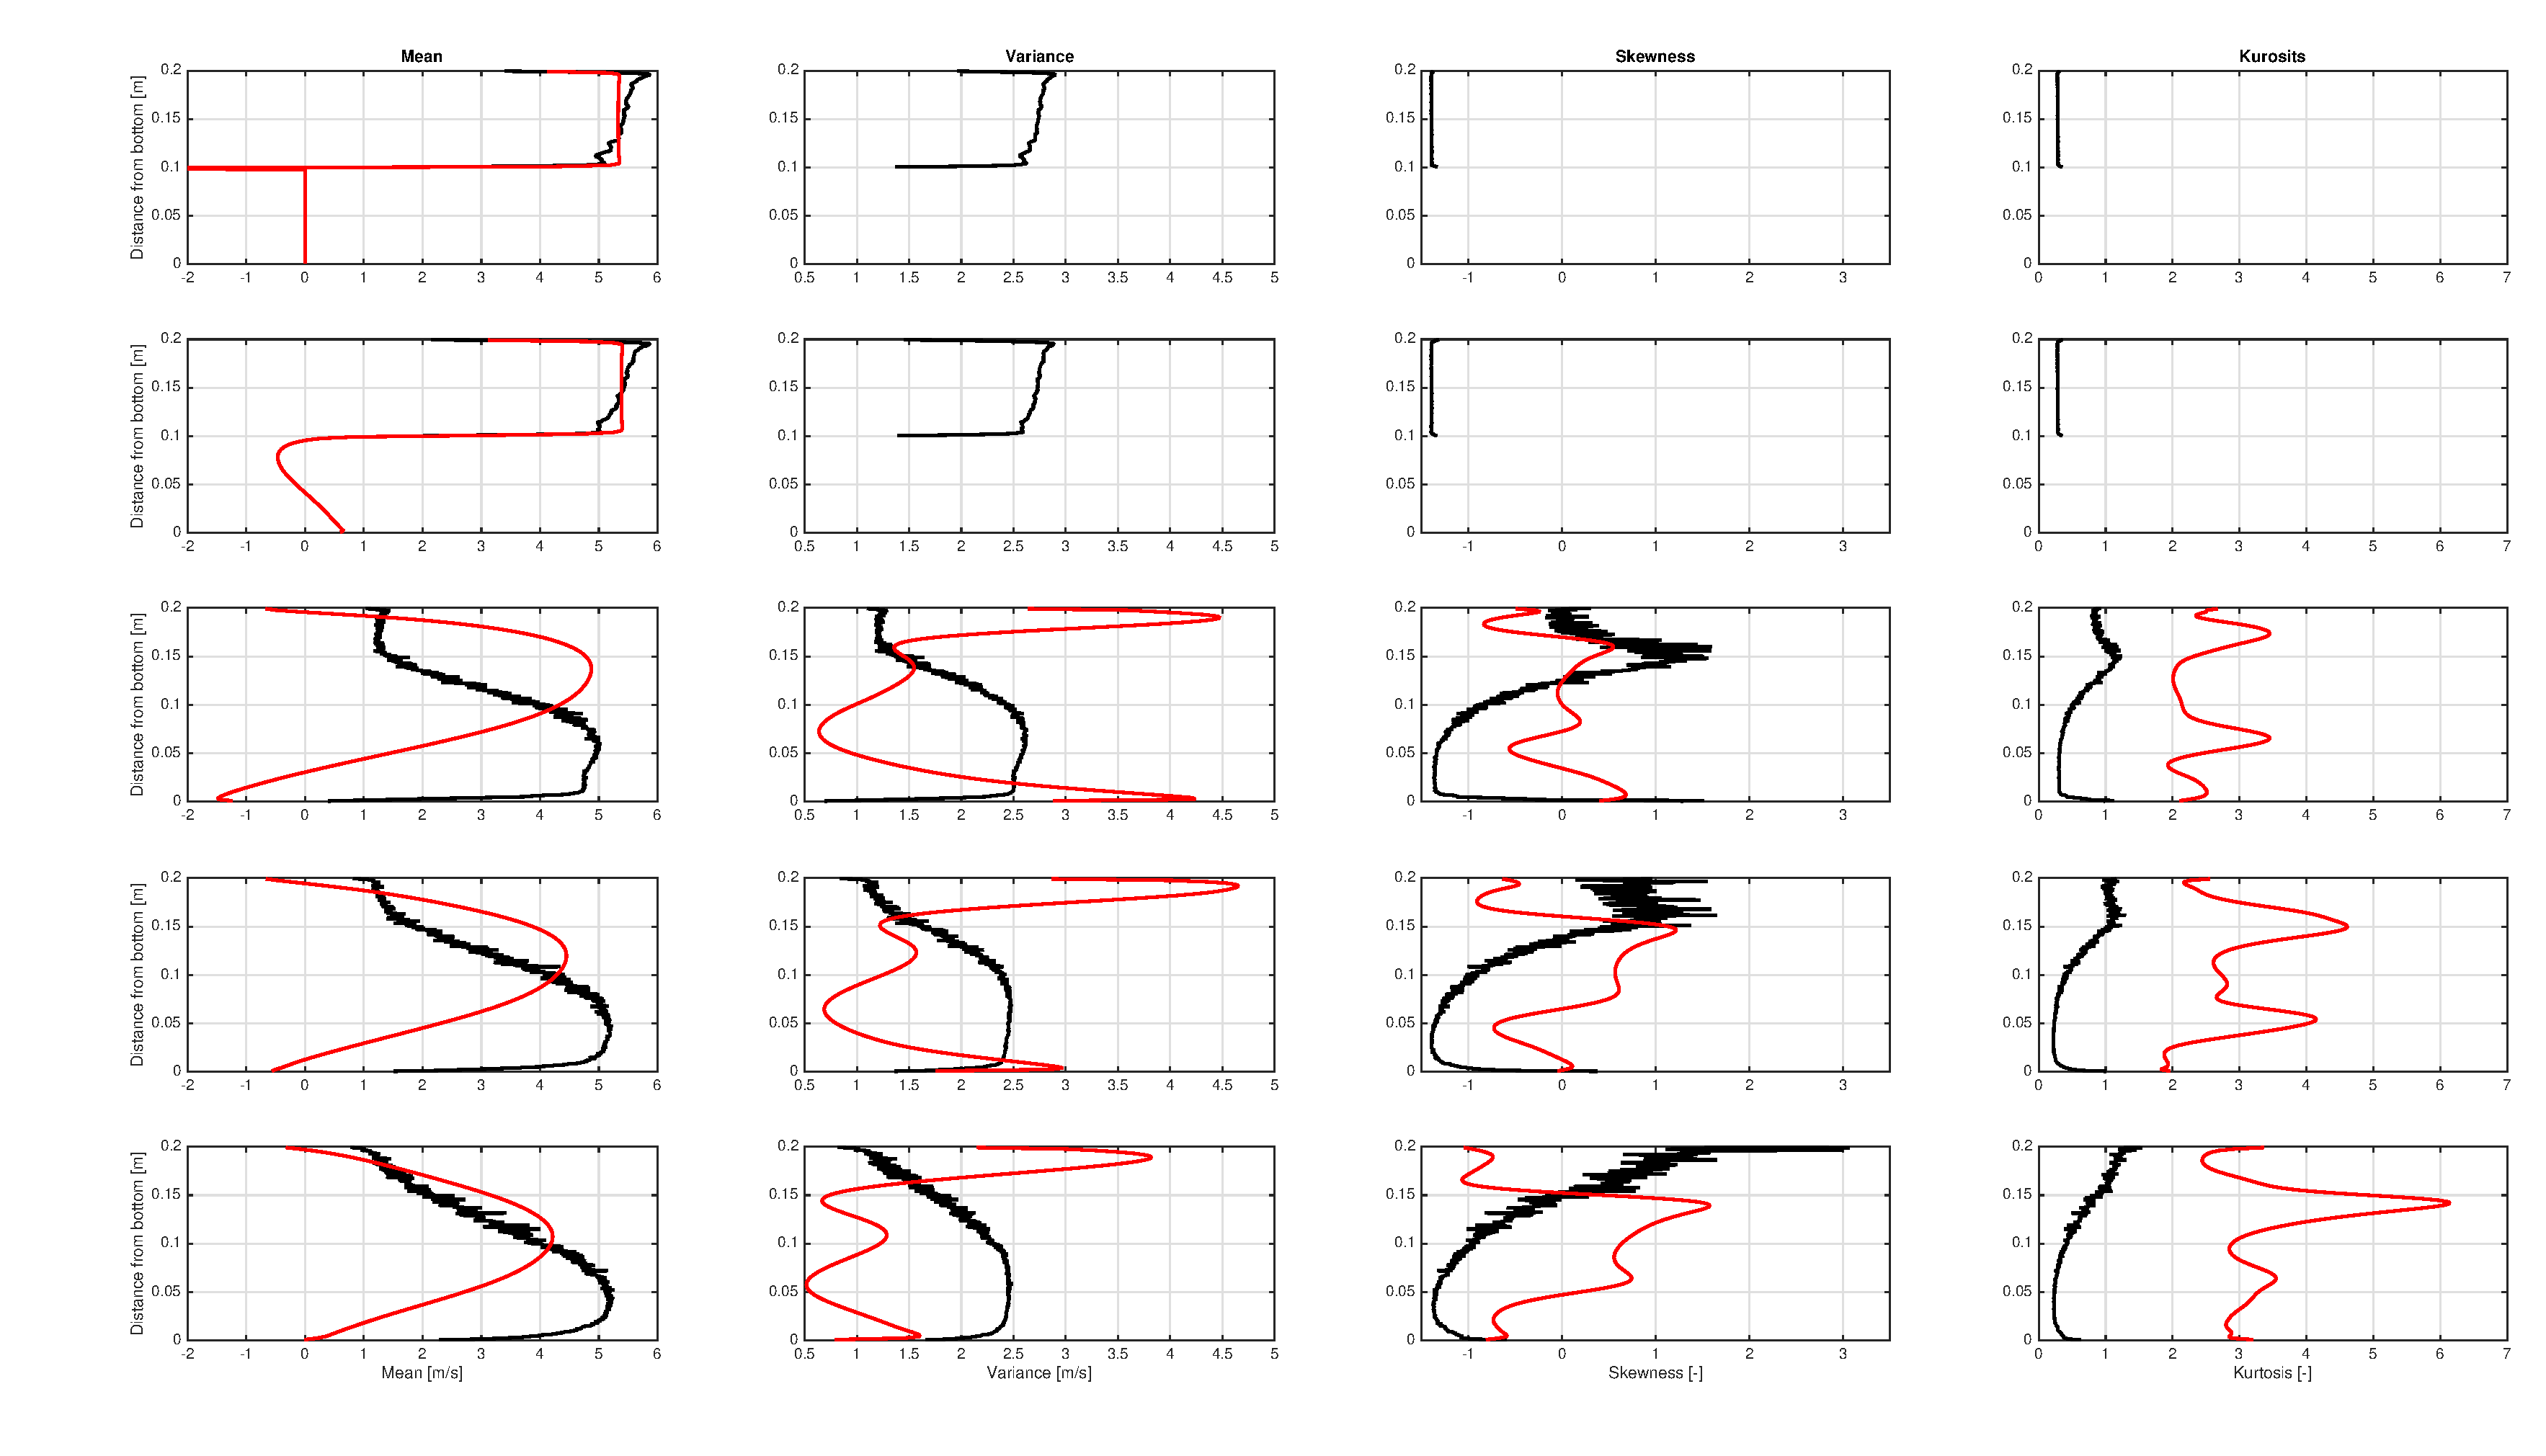
\includegraphics[trim=0 0 0 0,clip,angle=90,width=0.8\textwidth]{FIGURES/Re01_dns.eps}
\caption{Stochastic analysis and comparison for $u=5.295m/s$ for different x-positions}
\label{fig:bfsB}
\end{figure} 

\begin{figure}[!htb]
\centering
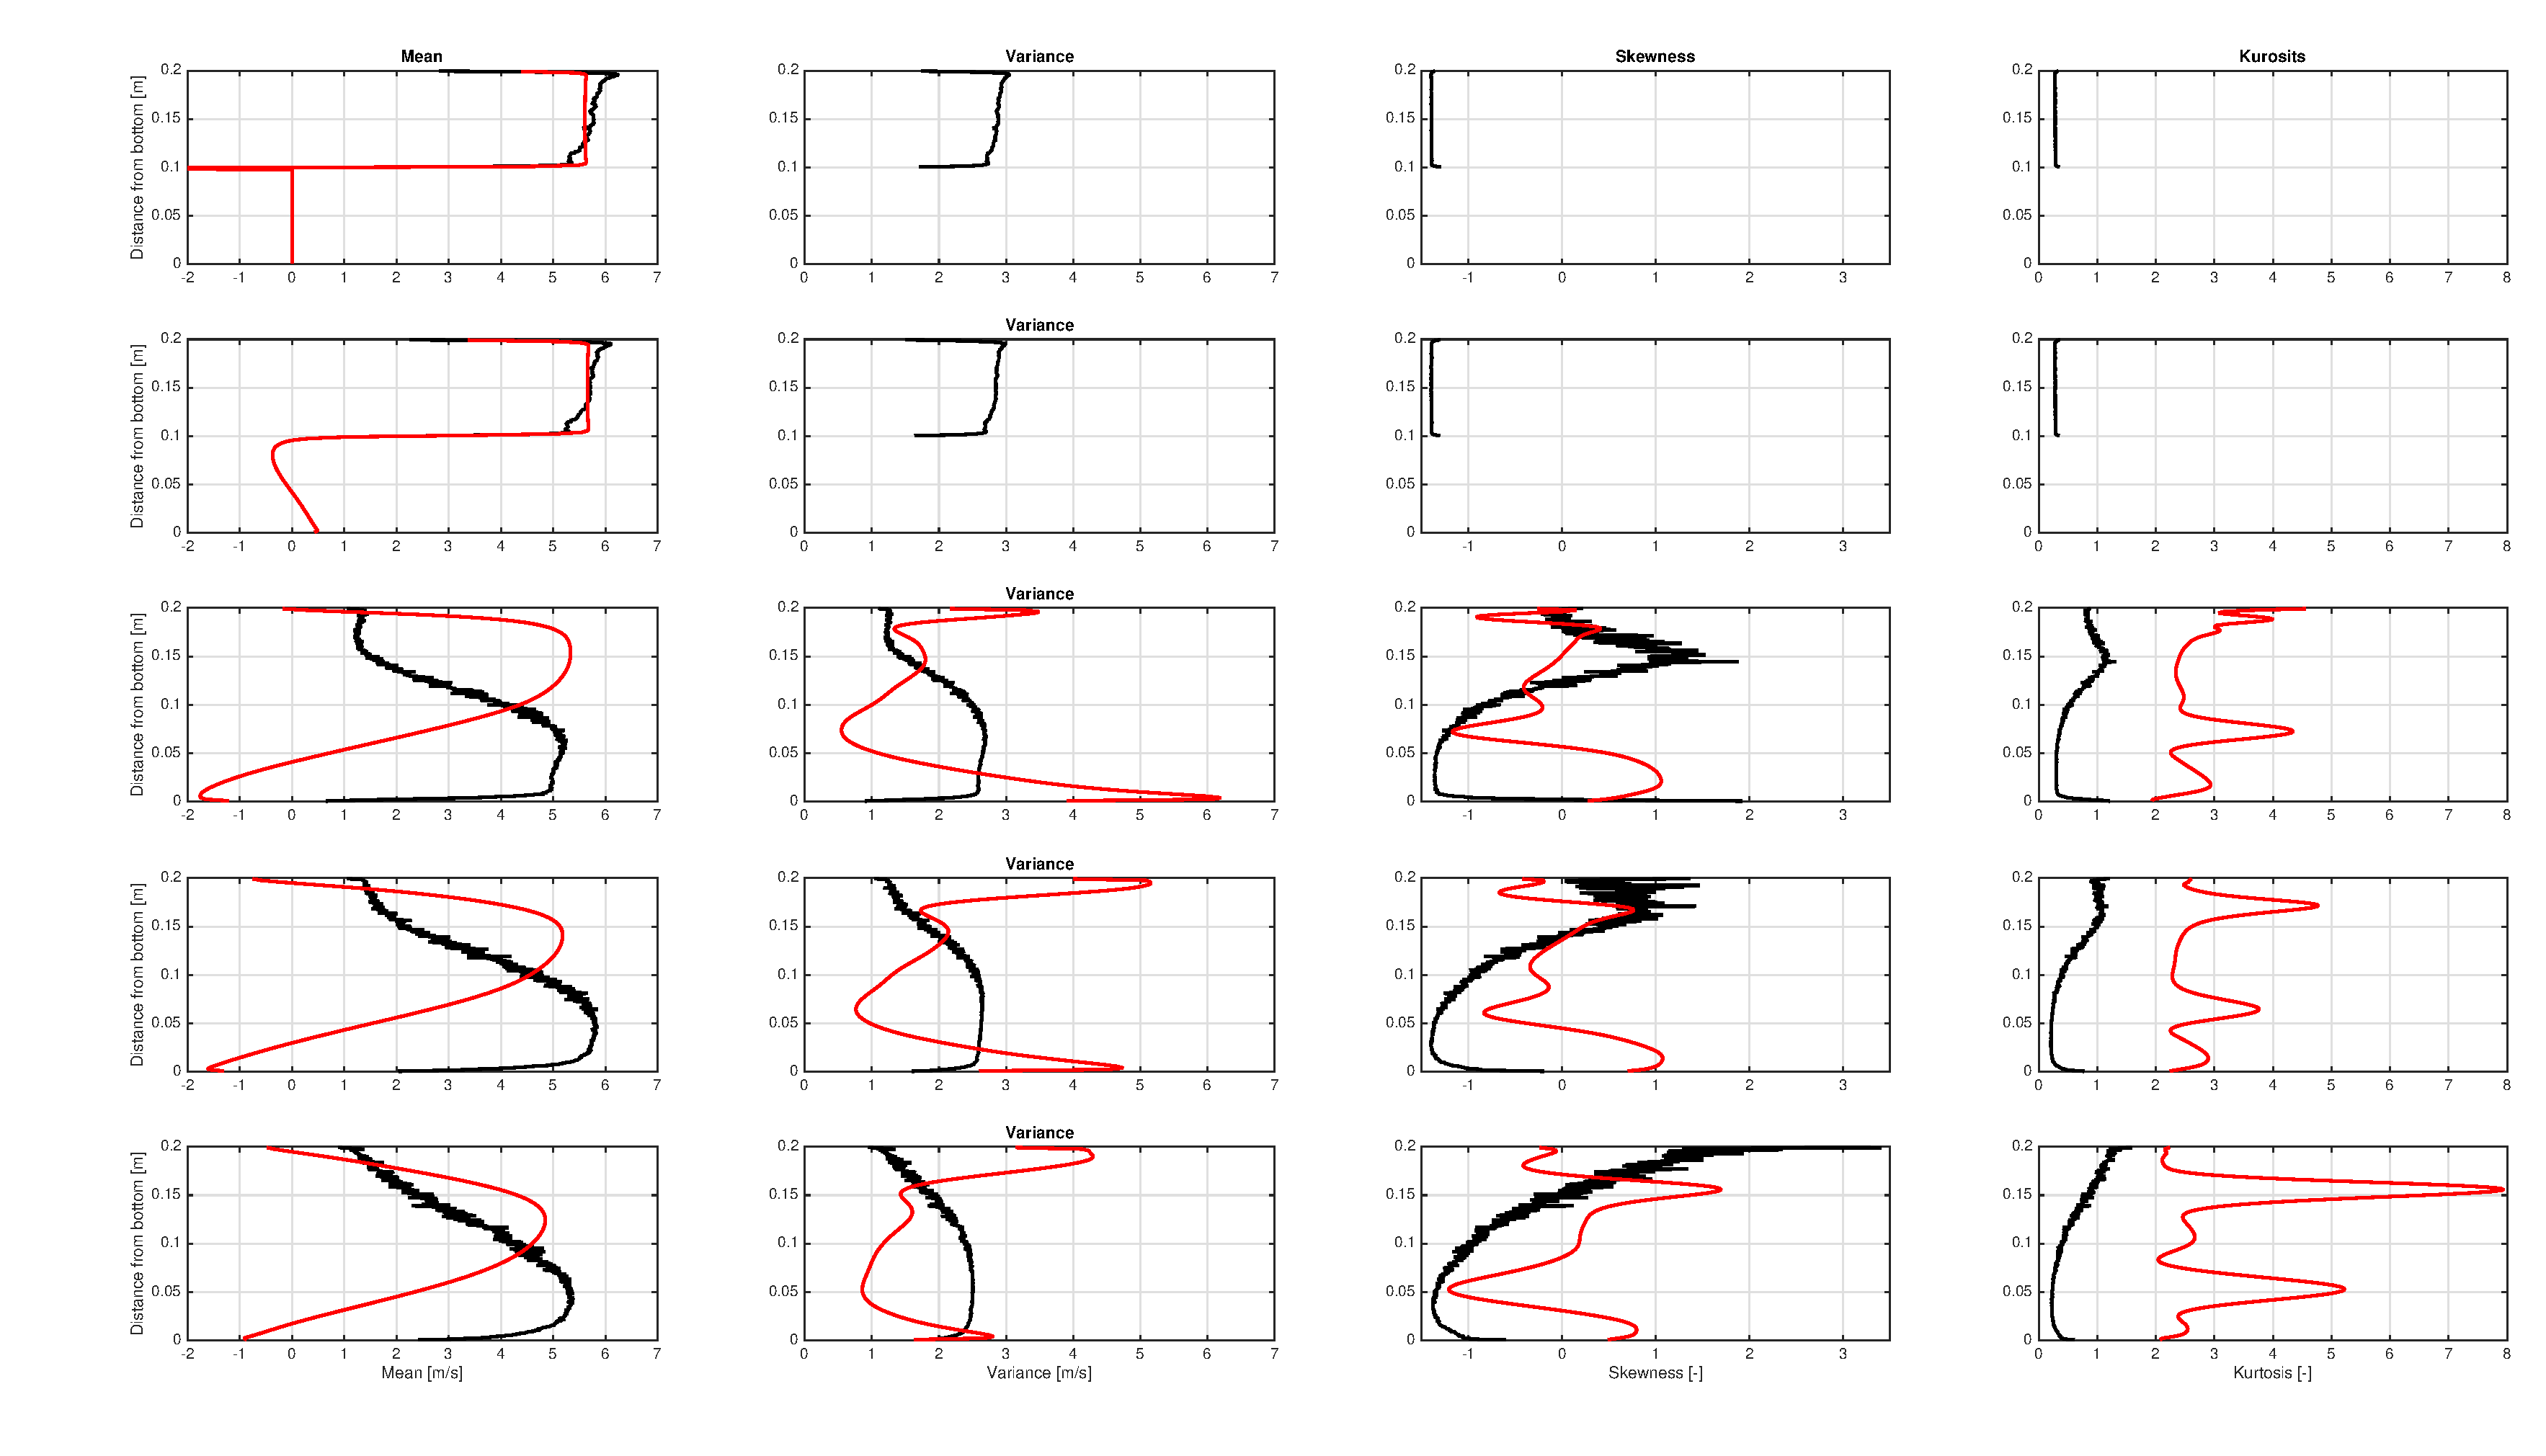
\includegraphics[trim=0 0 0 0,clip,angle=90,width=0.8\textwidth]{FIGURES/Re02_dns.eps}
\caption{Stochastic analysis and comparison for $u=5.579m/s$ for different x-positions}
\label{fig:bfsC}
\end{figure} 

\clearpage
\subsubsection*{Turbulent simulations}

A simulation of the given backward facing step was performed with the algebraic and the \ke\, turbulence model for $u=5.579m/s$. In none of the simulations, instabilities were encountered. No stochastic analysis was needed.

\noii The tendency that the jet is preferring the bottom wall could not be encountered in this simulations either (see figure~\ref{fig:bfsprofile}).

\begin{figure}[!htb]
\centering
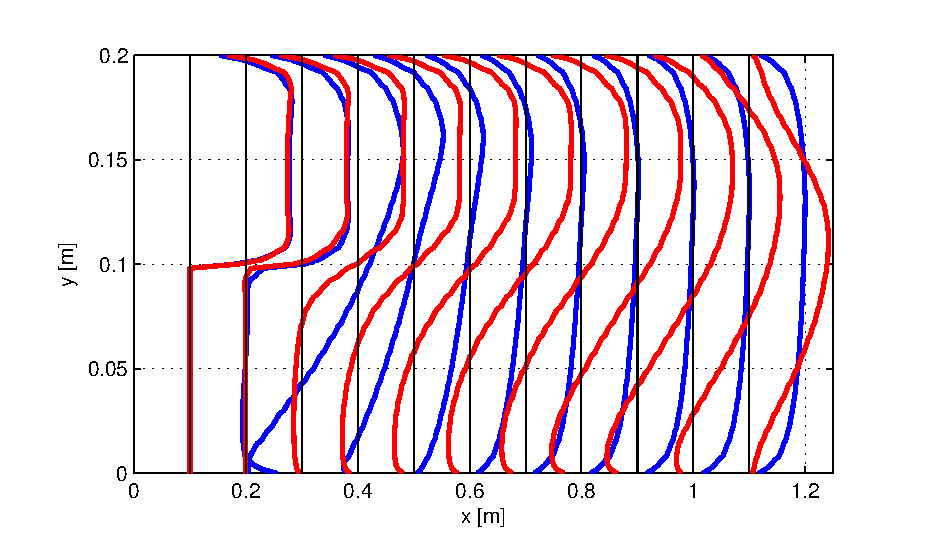
\includegraphics[trim=0 0 0 0,clip,width=0.8\textwidth]{FIGURES/bfs-profile.eps}
\caption{Velocity component in x-direction for (blue) algebraic and (red) \ke-simulation}
\label{fig:bfsprofile}
\end{figure} 



\noii The reattachment occurs in the algebraic simulation between position C and D and in the \ke\,simulation far behind E. The unsatisfying result of the \ke\,simulation might be due to an underestimated eddy viscosity directly behind the step corner due to a limitation of $\nu_T<\nu\cdot 100$ (see figure~\ref{fig:bfsnut}).

\begin{figure}[!htb]
\centering
\includegraphics[trim=0 200 0 200,clip,width=1.0\textwidth]{FIGURES/bfs-aturb.png}
\includegraphics[trim=0 200 0 200,clip,width=1.0\textwidth]{FIGURES/bfs-ke.png}
\caption{Contour plot of the eddy viscosity (top: algebraic, bottom: \ke)}
\label{fig:bfsnut}
\end{figure} 

% subsection backward_facing_step (end)

\clearpage
\section{K\'{a}rm\'{a}n vortex street - flow around a cylinder in a channel} % (fold)
\label{sec:karman_vortex_street_flow_around_a_cylinder_in_a_channel}

A cylinder (2D) was used to test how well the import of an arbitrary geometry works. The flow pattern in the wake of the cylinder is a well known and well studied phenomenon (K\'{a}rm\'{a}n vortex street). Measurements from an experiment conducted in a G\"ottingen-type wind tunnel during the lab course 'Praktikum Experimentelle Str\"omungsmechanik' 2015 was used to test the results for validity (see \citep{koehler2015}).

\noii The results of two simulation are presented here. The setup is chosen according to the experimental setup. The two simulations differ only in the chosen scenario: 1) channel and 2) free. It was seen that the chosen boundary conditions have clear influence on the flow patterns\footnote{It was not possible to simulate a big enough flow field, so that no influence of the boundary conditions could be noticed: the code needs to be extended for parallel simulations to be able to handle an appropriate mesh size.}.




\begin{center}
\begin{tabular}{lccc}
\hline 
Re                   & 61814\\      
Uniform velocity profile $u$         & 10 \\
Geometry (Flow field)  &  1$\times$0.2\\
Geometry (Cylinder)  &  x=0.2, y=0.1, d=0.03\\
Mesh Type & uniform \\
Mesh      & 256\,$\times$\,256 \\\hline 
\end{tabular}
\end{center}

\noii The 'animation' figure~\ref{fig:karman-ani1} shows how the flow develops from the initial condition (no flow) to the periodic flow condition with well visible vortex street  and \ref{fig:karman-ani2} shows a fully developed vortex street. The vortex shedding frequency matches well with the expected value:
\begin{align*}
f=\frac{Sr \cdot u}{d}=66.7Hz \qquad \text{with } Sr\approx0.2
\end{align*}

\noii Figure~\ref{fig:karman-stoch2} shows the stochastic analysis along a path downstream of cylinder with a distance $\Delta x = 0.100$. The stochastic analysis of the measured values are plotted in figure~\ref{fig:karman-stoch1}. The overall tendencies of the modes are both in the simulation and in the measurements similar. The influence of the boundary conditions is clearly visible leading to the discrepancies. For detailed evaluation of the experimental results (among other things modes along a path behind a cylinder) we would like to refer interested reader to \citep{koehler2015}. 

\newcommand{\inkarman}[1]{\includegraphics[trim=0 250 0 250,clip,width=0.8\textwidth]{#1}}

\begin{figure}[!htb]
\centering
\inkarman{FIGURES/karman10.png}
\inkarman{FIGURES/karman20.png}
\inkarman{FIGURES/karman30.png}
\inkarman{FIGURES/karman40.png}
\inkarman{FIGURES/karman50.png}
\inkarman{FIGURES/karman60.png}
\inkarman{FIGURES/karman70.png}
\caption{First 70ms with a sample rate of 100Hz}
\label{fig:karman-ani1}
\end{figure} 

\begin{figure}[!htb]
\centering
\inkarman{FIGURES/k1000.png}
\inkarman{FIGURES/k1001.png}
\inkarman{FIGURES/k1002.png}
\inkarman{FIGURES/k1003.png}
\inkarman{FIGURES/k1004.png}
\inkarman{FIGURES/k1005.png}
\inkarman{FIGURES/k1006.png}
\caption{Fully developed vortex street: part of a full periode (sample rate 100Hz)}
\label{fig:karman-ani2}
\end{figure} 

\begin{figure}[!htb]
\centering
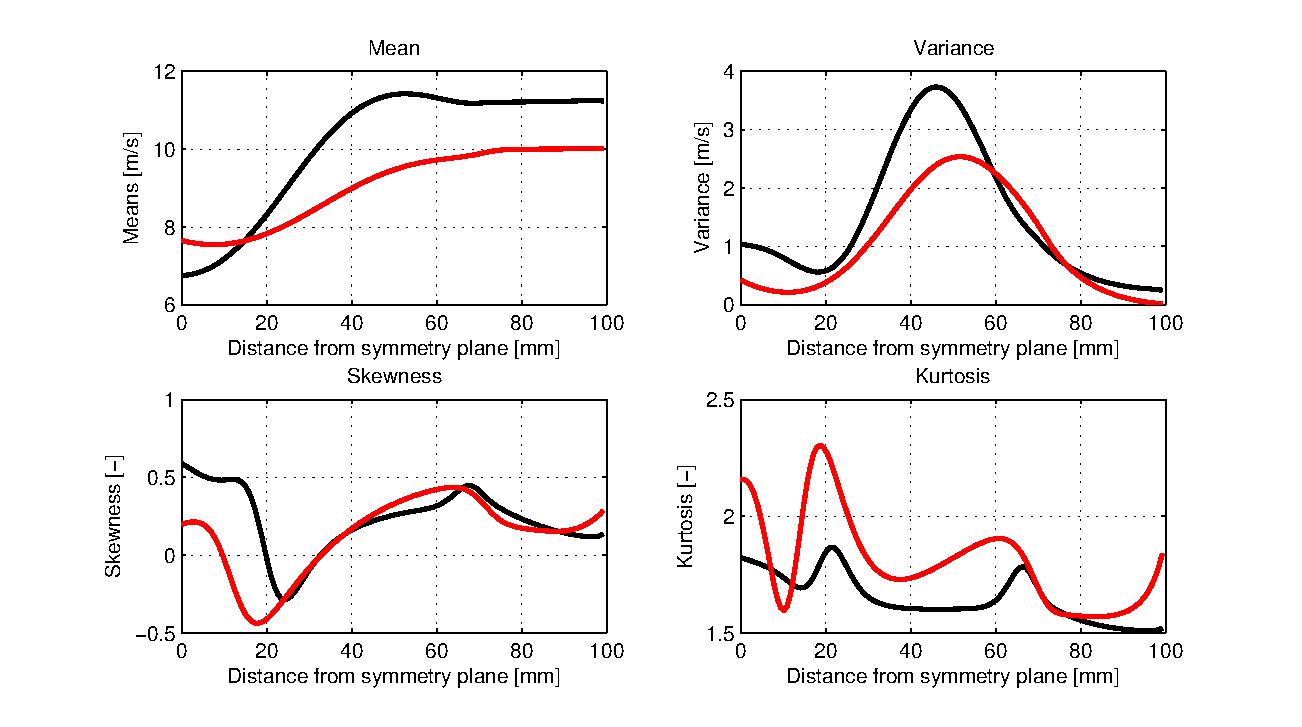
\includegraphics[trim=10 0 10 0,clip,width=1.0\textwidth]{FIGURES/karman-stoch.eps}
\caption{Stochastic analysis of the simulation results along a path 100mm behind the cylinder (black: channel, red: free)}
\label{fig:karman-stoch2}
\end{figure} 


\begin{figure}[!htb]
\centering
\includegraphics[trim=80 0 80 0,clip,width=1.0\textwidth]{FIGURES/wake-ana.png}
\caption{Stochastic analysis of the experimental measurement along a path 100mm behind the cylinder}
\label{fig:karman-stoch1}
\end{figure} 





% subsection karman_vortex_street_flow_around_a_cylinder_in_a_channel (end)

% chapter numerical_results (end)
%!TEX root = ./../projectReport.tex

\chapter{Usability} % (fold)
\label{cha:usability}
To perform the commands shown in this chapter please navigate to the C++-project folder ('turbulence').


\section{Project folder} % (fold)
\label{sec:project_folder}

NS-EOF can still be run by writing into the shell the following command:

\bashh{SCENARIOS/run.txt}{1}

\noii However, we advice to run the Python-script 'run' both on the cluster and locally to start a simulation\footnote{For more informations on the options we refer to the help:
\bashh{SCENARIOS/runh.txt}{1}
}:

\bashh{SCENARIOS/runl.txt}{1}

\noii By doing so, the simulation is started but also a new folder is created containing all relevant file of a simulation. This folder may be referenced in the following as project folder.

\noii By copying and placing all the input files (configuration file, backup file for initialisation, geometry file) and result files (output, vtk files, backup file, timing results) into one folder the user is enabled to completely understand the simulation at a later time.

\noii The following tree shows the structure of the project folder:
\dirtree{%
.1 project.
.2 job.cmd.
.2 log.
.2 out.
.2 petsc\_commandline\_arg.
.2 scenario.xml.
.2 timing/.
.3 ....
.2 vtks/.
.3 ....
}

\noii The next sections describe two input files (configuration and geometry files) in more detail.

\clearpage

\section{Configuration file} % (fold)
\label{sec:configuration_file}

For completeness reasons a configuration file in its original appearance as provided at the beginning of the lab course is shown. 

\noii It contains the setup for a DNS simulation of a backwards facing step scenario with a streched mesh.

\xmll{SCENARIOS/conf-reference.xml}{2}

\noii All additional new options are shown in the following sections in reference to this file.

\newpage
\subsubsection*{Algebraic Turbulence Model}

For the second worksheet the group implemented an algebraic turbulence model with different methods to limit the mixing length and thus the eddy viscosity (nulimiter=1: no limitation; =3 limitation with the help of a laminar flat plate Blasius boundary layer; =4 limitation with the help of a turbulent flat boundary layer). 

\xmll{SCENARIOS/type-aturb.xml}{2}

\noii A laminar simulation with this implementation can be performed by setting $\nu_t$ to zero (type='laminar'). The results should be comparable with the DNS-simulation (see [LMS-15, S.XY]).  

\subsubsection*{k-$\varepsilon$-Turbulence Model}

The user can use alternatively to the algebraic turbulence model the k-$\varepsilon$ model to calculate the eddy viscosity. Following optional parameters can be set:
\begin{itemize}
\item model constants $C_{\varepsilon 1}$, $C_{\varepsilon 2}$, $\sigma_k$, $\sigma_\varepsilon$ and $C_{\mu}$ (see equation XY)
\item wall near treatment (model=0: no wall modifications, =1: Lam and Bremhorst, =2: Chien, =3: Jones and Launder, =4 Fan and Lakshminarayana)
\item adaptive time stepping (number of refinements and permitted error - see section XY)
\item solving quasi laminar for the first 'start' seconds (not solving the transport equations for $k$ and $\varepsilon$ and setting $\nu_T=0$)
\end{itemize}

\xmll{SCENARIOS/type-ke.xml}{2}

\noii A laminar simulation with this implementation can be performed by setting $\nu_t$ to zero (type='laminar'). The results should be comparable with the DNS-simulation (see [LMS-15, S.XY]).  

\subsubsection*{Scenarios}

As described in section~XY 3 additional scenarios were added:

\begin{itemize}
\item symmetrical channel
\xmll{SCENARIOS/scenario-channel-symm.xml}{1}
\item boundary layer over a flat plate
\xmll{SCENARIOS/scenario-boundary.xml}{1}
\item free shear flow (without any side walls)
\xmll{SCENARIOS/scenario-free.xml}{1}
\end{itemize}

\subsubsection*{Inlet}

For every scenario except for 'cavity' the velocity inlet profile in x-direction can be prescribed as either uniform (true) or parabolic (false).

\xmll{SCENARIOS/scenario-uniform.xml}{1}

\subsubsection*{Flow around Arbitrary Geometry}

The user can specify a reference to a geometry file (see XY) to be used as obstacle in any scenario.

\xmll{SCENARIOS/ageom.xml}{2}

\subsubsection*{Backup Files}

The user can specify the backup files to be used for initialisation and respectively for saving the results of the final time step.

\xmll{SCENARIOS/restart.xml}{2}

% subsection configuration_file (end)

\clearpage

\section{Geometry file} % (fold)
\label{sec:geometry_file}

The geometry file (.geo) contains the coordinated of all obstacle cells. Each line represents exactly one obstacle cell and has the following format (with the first number i, the second number j and the third number k):

\xmll{SCENARIOS/geo.txt}{2}

\noii The team created two Matlab-scripts for creating files of the necessary format for 2D geometries:
\begin{itemize}
\item \underline{Scripting}:\\
The user specifies with a basic function which position is in the geometry and which is in the flow field. The Matlab-script evaluates this function for the middle point of each cell and writes the file. Elementary geometries (circle, square, plate) and geometries composed by these can be created:

\begin{figure}[!htb]
\centering
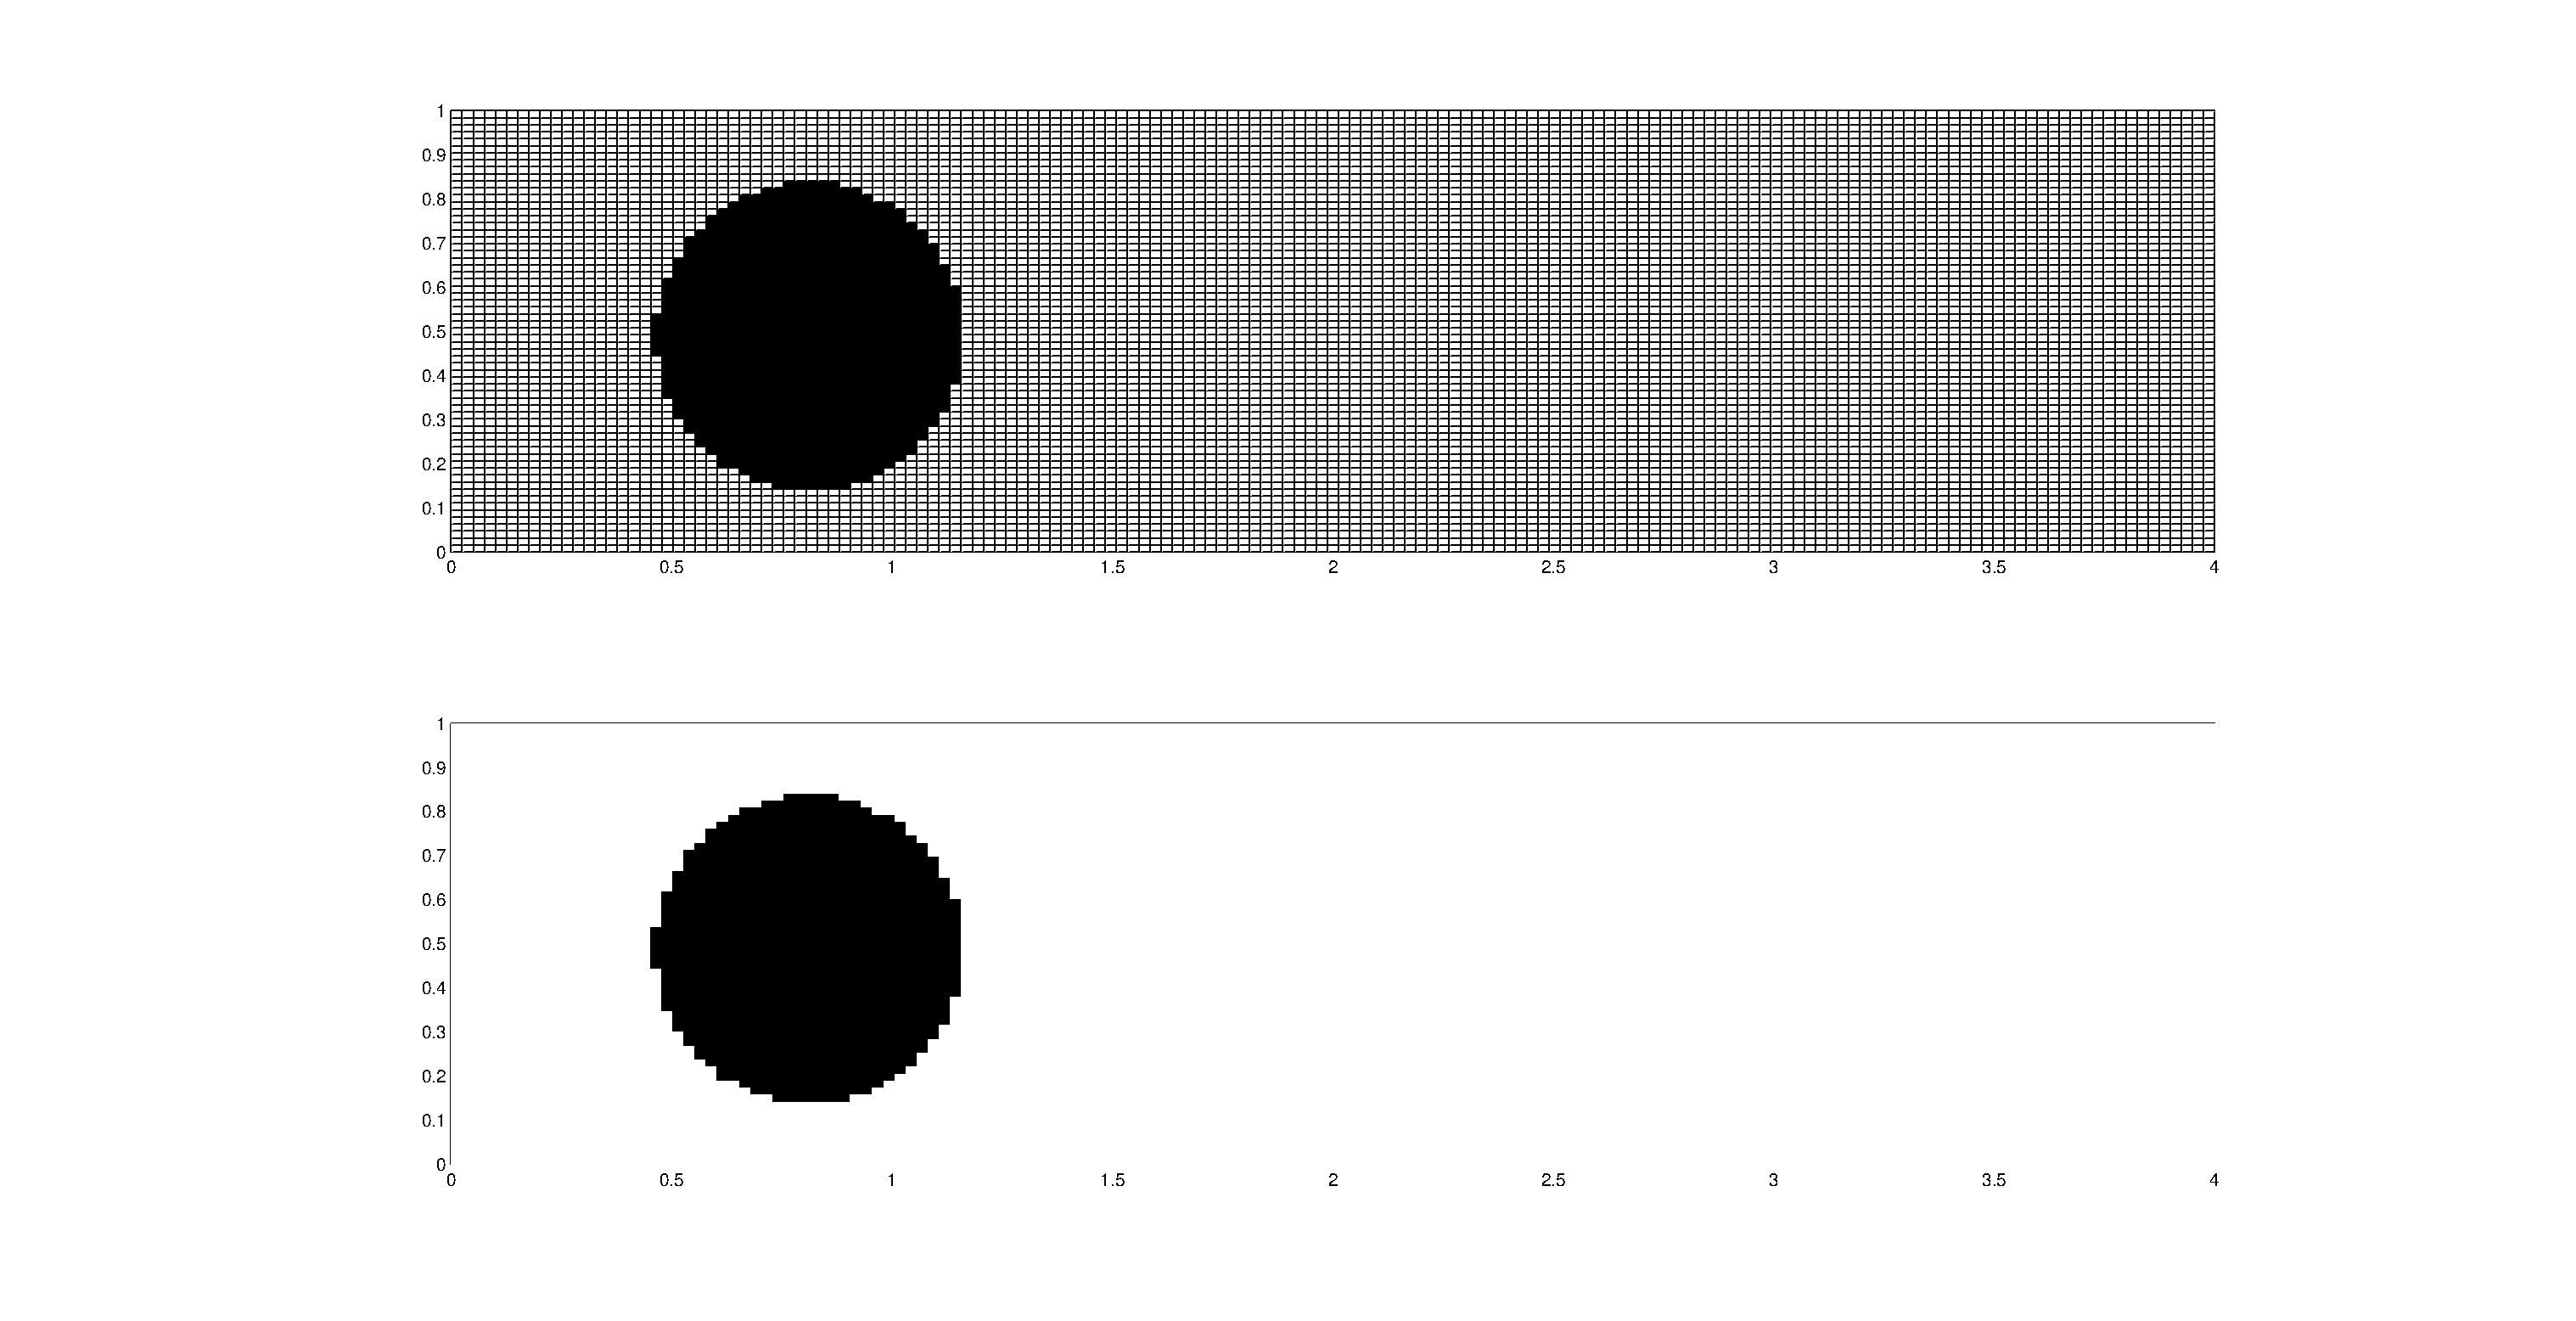
\includegraphics[scale=.3]{FIGURES/circle.eps}
\caption{Circle in a channel}
\label{fig:circle_in_channel}
\end{figure} 

\item \underline{Drag \& Drop}:\\
The user draws on a cartesian coordinate system the border of the geometry. The program decides recursively which cell is a obstacle cell which is a fluid cell.
\end{itemize}



% subsection geometry_file (end)

% chapter usability (end)
\chapter{Conclusion} % (fold)
\label{cha:conclusion}

% chapter conclusion (end)





\pagenumbering{roman}
\setcounter{page}{\thealteSeitenzahl}
\appendix
%\begin{appendices}

\chapter{APPENDIX} % (fold)
\label{cha:details_concerning_consistent_linearization_of_2d_mortar_contact}


\end{appendices}

%\listoffigures
\bibliography{projectReport}{}
%\bibliography{my_bachelor_thesis}{}
\bibliographystyle{plainnat}
%\bibliography{my_bachelor_thesis}{}
%\bibliographystyle{plainnat}

\end{document}

%%%%%%%%%%%%%%%%%%%%%%%%%%%%%%%%%%%%%%%%%%%%%%%%%%%%%%%%%%%%%%%%%%%%%%%
%%%%%%%%%%%%%%%%%%%%%%%%%%%%             %%%%%%%%%%%%%%%%%%%%%%%%%%%%%%
%%%%%%%%%%%%%%%%%%%%%%%%%%%% end of file %%%%%%%%%%%%%%%%%%%%%%%%%%%%%%
%%%%%%%%%%%%%%%%%%%%%%%%%%%%             %%%%%%%%%%%%%%%%%%%%%%%%%%%%%% 
%%%%%%%%%%%%%%%%%%%%%%%%%%%%%%%%%%%%%%%%%%%%%%%%%%%%%%%%%%%%%%%%%%%%%%%